% Optimally you should use XeLaTeX to typeset it, using system fonts. If you use pdflatex, standard LaTeX sans fonts will be used instead.
%
% This makes use of some stock MultiMarkdown LaTeX boilerplate. Thanks go to Fletcher Penney for creating a useful and simple system to extend from.

\documentclass[oneside,article,14pt,dvipsnames]{memoir}

\usepackage{layouts}[2001/04/29]
\usepackage[svgnames]{xcolor}
\definecolor{coolgrey}{Hsb}{293, 0.0, 0.5}
\definecolor{plumbgrey}{Hsb}{314, 0.3, 0.5}
\definecolor{redgrey}{Hsb}{337, 0.31, 0.6}
\usepackage{url,verse}
\usepackage{wrapfig}
\usepackage{sectionbreak}
\usepackage{perpage} %the perpage package
\MakePerPage{footnote} %the perpage package command
\usepackage{xpatch}
\usepackage{fancyvrb}
\usepackage{adjustbox}
\usepackage[esperanto]{babel}
\usepackage{amssymb}
\usepackage[utf8]{inputenc}
\usepackage[labelformat=empty]{caption}
\usepackage{calligra}
\usepackage{tikz}
\usetikzlibrary{matrix,fit,chains,calc,scopes}            
\usepackage{tcolorbox}
\tcbuselibrary{skins}
\usepackage{auto-pst-pdf} %To compile psvectorian directly
\usepackage{psvectorian}
\usepackage[all]{nowidow}
\usepackage[acronym, toc]{glossaries}

\newacronym{vd}{vd.}{vidu}

\glstoctrue
\makeglossaries
\makeindex

\usepackage{pdfpages}
\usepackage[T1]{fontenc}
\usepackage{fontenc,unicode-math}

%\usepackage{fontspec}
\setmainfont[Ligatures=TeX]{TeX Gyre Schola}
%\usepackage{beton}
%\renewcommand{\bfdefault}{sbc}
\usepackage[scale=0.89]{tgheros} % Helvetica is too big


%	\renewcommand{\familydefault}{\sfdefault}
	\newcommand{\helvetican}{}
	\newcommand{\helveticanl}{}

% Body Text Formatting
\linespread{1.2}
\setlength{\abnormalparskip}{0.5em}
\setlength{\parindent}{1.5em}


% Footnotes
\setlength{\footmarkwidth}{1.8em}
\setlength{\footmarksep}{0em}
\footmarkstyle{\footnotesize{#1}.\hfill}
\setfootins{16pt}{16pt}
\setlength{\footnotesep}{16pt}


%
%	8.5 x 11 layout for memoir-based documents
%   As defined in the stock MultiMarkdown system
%
%%% need more space for ToC page numbers
\setpnumwidth{2.55em}
\setrmarg{3.55em}

%%% need more space for ToC section numbers
\cftsetindents{part}{0em}{3em}
\cftsetindents{chapter}{0em}{3em}
\cftsetindents{section}{3em}{3em}
\cftsetindents{subsection}{4.5em}{3.9em}
\cftsetindents{subsubsection}{8.4em}{4.8em}
\cftsetindents{paragraph}{10.7em}{5.7em}
\cftsetindents{subparagraph}{12.7em}{6.7em}

%%% need more space for LoF numbers
\cftsetindents{figure}{0em}{3.0em}

%%% and do the same for the LoT
\cftsetindents{table}{0em}{3.0em}

%%% set up the page layout
\settrimmedsize{\stockheight}{\stockwidth}{*}	% Use entire page
\settrims{0pt}{0pt}

% Comment out the following command and replace it with the second, below it, if you intend to use CriticMarkup's margin notes, or marginalia of any sort.
\setlrmarginsandblock{1in}{1in}{*}
% \setlrmarginsandblock{1in}{2.5in}{*}
\setulmarginsandblock{1in}{1in}{*}

\setmarginnotes{17pt}{1.5in}{\onelineskip}
\setheadfoot{\onelineskip}{2\onelineskip}
\setheaderspaces{*}{2\onelineskip}{*}
\checkandfixthelayout

\usepackage{fancyvrb}
\usepackage{graphicx}
\usepackage{booktabs}
\usepackage{tabulary}
%\usepackage{listings}
\usepackage[sort&compress]{natbib}
\usepackage[normalem]{ulem}

\renewcommand{\contentsname}{TABELO DE ENHAVO}


% Make use of MultiMarkdown's CriticMarkup support for proofing notations
% If you have installed your own copy of MMD, you should use the second command instead.
\input{/Applications/Scrivener.app/Contents/Resources/MultiMarkdown/latex-support/mmd6-criticmarkup}
% \input{mmd6-criticmarkup}

\VerbatimFootnotes

% Section Headings
\setsecheadstyle{\helveticanl\LARGE\raggedright\textcolor{ForestGreen}}
\setsubsecheadstyle{\helveticanl\large\raggedright\textcolor{ForestGreen}}
\setsubsubsecheadstyle{\helveticanl\normalsize\raggedright\textcolor{ForestGreen}}

\maxsecnumdepth{chapter}
\setsecnumdepth{chapter}
\settocdepth{section}

% Spacing Model
% Use "negative" values for the beforeXskip settings; this indicates the following paragraph should have its indent suppressed.
\setbeforesecskip{-14pt}
\setaftersecskip{12pt}
\setbeforesubsecskip{-14pt}
\setaftersubsecskip{12pt}
\setbeforesubsubsecskip{-14pt}
\setaftersubsubsecskip{6pt}

% Chapter heading style
\makechapterstyle{modern-style}{
    \renewcommand*{\chaptitlefont}{\helveticanl\huge\centering\normalfont}
    \renewcommand*{\chapnumfont}{\helvetican\Huge\raggedright\mdseries}
	\renewcommand*{\chapnamefont}{\chapnumfont}
	\renewcommand*{\printchaptername}{\newpage\chapnamefont\color{ForestGreen}}
	\renewcommand*{\printchapternum}{}
	\setlength{\beforechapskip}{36pt}
    \setlength{\afterchapskip}{12pt}
	\setlength{\midchapskip}{6pt}
	\setlength{\midchapskip}{6pt}
}
\chapterstyle{modern-style}

% Part Breaks
\renewcommand{\parttitlefont}{\helvetican\huge\raggedright\normalfont\color{ForestGreen}}
%\renewcommand{\partnamefont}{\helvetican\fontsize{30pt}{30pt}\raggedright\mdseries\color{ForestGreen}}
\renewcommand{\partnamefont}{}
\renewcommand{\printpartname}{}
\renewcommand{\printpartnum}{}
\renewcommand{\partnumfont}{\partnamefont}
\renewcommand{\beforepartskip}{\null\vfil\thispagestyle{empty}}
\renewcommand{\midpartskip}{\par\vspace{6pt}}
% Comment the following line if you wish to print the name of the part
\renewcommand{\printparttitle}{\chapnamefont\centering\color{ForestGreen}}
\renewcommand{\afterpartskip}{\par\vspace{6pt}}


\renewcommand{\cftpartleader}{\cftdotfill{\cftdotsep}}
\renewcommand{\cftchapterleader}{\cftdotfill{\cftdotsep}}

\pagestyle{plain}


\renewcommand{\sectionbreak}{\fancybreak{\color{ForestGreen}\textbf{\star}}}
\def\mytitle{Kudra kaj trika terminaro}
\def\myauthor{Myrtle Verda}
% Set up PDF
\usepackage[
	plainpages=false,
	colorlinks=true,
	    unicode=true,          % non-Latin characters in Acrobat’s bookmarks
	urlcolor=ForestGreen,
	linkcolor=ForestGreen,
	citecolor=ForestGreen,
	filecolor=ForestGreen,
	pdfpagelabels,
	pdftitle={\mytitle},
	pagebackref,
	pdfauthor={\myauthor},
	bookmarksnumbered=true,
	bookmarksopen=true
	]{hyperref}
\hypersetup{bookmarksdepth=3}
\usepackage{memhfixc}

%
%	Configure information from metadata for use in title
%   Using default MultiMarkdown methods

\ifx\latexauthor\undefined
\else
	\def\myauthor{\latexauthor}
\fi

\ifx\subtitle\undefined
\else
%	\addtodef{\mytitle}{}{ \\ \subtitle}
	\expandafter\def\expandafter\mytitle\expandafter{\mytitle \\ \subtitle}
\fi

\ifx\affiliation\undefined
\else
%	\addtodef{\myauthor}{}{ \\ \affiliation}
	\expandafter\def\expandafter\myauthor\expandafter{\myauthor \\ \affiliation}
\fi

\ifx\address\undefined
\else
%	\addtodef{\myauthor}{}{ \\ \address}
	\expandafter\def\expandafter\myauthor\expandafter{\myauthor \\ \address}
\fi

\ifx\phone\undefined
\else
%	\addtodef{\myauthor}{}{ \\ \phone}
	\expandafter\def\expandafter\myauthor\expandafter{\myauthor \\ \phone}
\fi

\ifx\email\undefined
\else
%	\addtodef{\myauthor}{}{ \\ \email}
	\expandafter\def\expandafter\myauthor\expandafter{\myauthor \\ \email}
\fi

\ifx\event\undefined
\else
	\date[\mydate]{\today}
\fi

\ifx\latextitle\undefined
	\def\latextitle{\mytitle}
\else
\fi
 %   remove figure captions

% http://tex.stackexchange.com/a/58638/5764
\makeatletter
\def\ifemptyarg#1{%
	\if\relax\detokenize{#1}\relax % H. Oberdiek
	\expandafter\@firstoftwo
	\else
	\expandafter\@secondoftwo
	\fi}
\makeatother

\let\oldcaption\caption
\AtBeginDocument{%
	\renewcommand{\caption}[2][]{%
		\ifemptyarg{#2}{}{\oldcaption[#1]{#2}}%
	}%
}
\date{}

\renewcommand*{\psvectorianDefaultColor}{ForestGreen}%

\tcbset{
	Baystyle/.style={
		sharp corners,
		enhanced,
		boxrule=6pt,
		colframe=ForestGreen,
		height=\textheight,
		width=\textwidth,
		borderline={8pt}{-11pt}{},
	}
}


\title{\mytitle}
\author{\myauthor}

\begin{document}


\begin{tcolorbox}[Baystyle,]
	{\begin{center}
			\vspace*{0.14\textheight}
			\fontsize{45}{45}\scshape \mytitle\\        
			\vspace*{0.018\textheight}
			%\vspace*{0.2\textheight}
			% Big Logo\\
			\begin{center}
			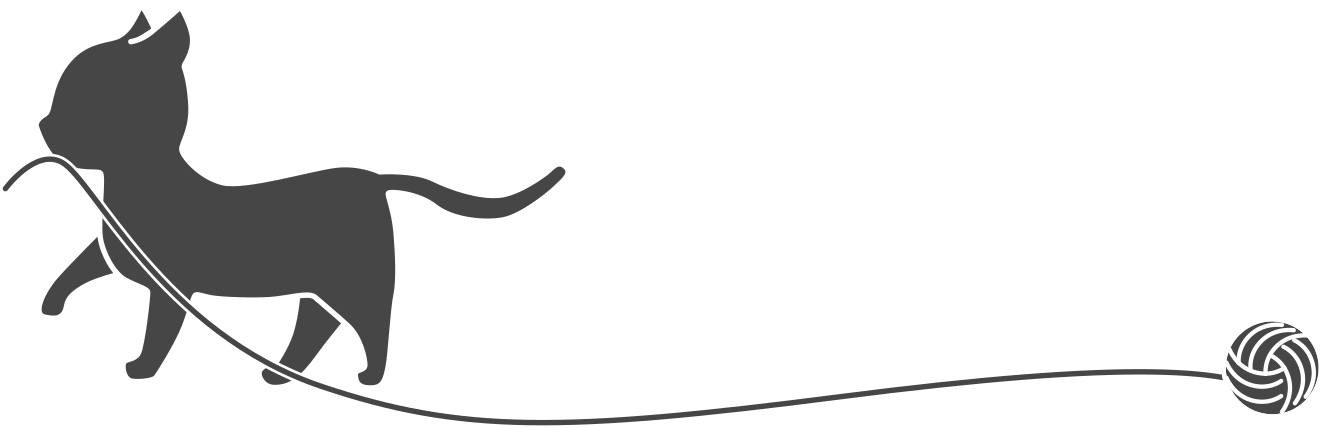
\includegraphics[width=0.5\textwidth]{cat-wool-line-clipart.png}
			\end{center}
			\vspace*{0.02\textheight}
			{\fontsize{12}{12}\calligra }
			\fontsize{28}{28}\scshape \myauthor\\
			\vspace*{0.1\textheight}
			\centering
			\begin{tikzpicture}[
				start chain=main going right,
				]
				\node[on chain,align=center,draw=none] (a1){{\fontsize{12}{12}\calligra %Illustrations by%
					} \\
					{\Large %Designer
					}
				}; 
				{ [start branch=A going below]
					\node[on chain,align=center,draw=none,scale=0.01](d1){};
					\node[on chain,align=center,draw=none,](d2){\Huge };
					%\node[on chain,align=center,draw=none,scale=0.01](d3){};
				}
				\node[on chain,align=center,draw=none,scale=1] (a2){\psvectorian[scale=0.3]{87}\psvectorian[scale=0.3,mirror]{87}}; 
				{ [start branch=B going below]
					\node[on chain,align=center,draw=none,scale=0.01](s1){};
					\node[on chain,align=center,draw=none,](s2){};
					%\node[on chain,align=center,draw=none,scale=0.01](s3){}; 
				}
				\node[on chain,align=center,draw=none]  (a3){{\fontsize{12}{12}\calligra %Final review by
					} \\
					{\Large %Revisor
					}
				};          
				{ [start branch=C going below]
					%\node[on chain,align=center,draw=none,scale=0.01](e1){};
					\node[on chain,align=center,draw=none,](e2){\Huge };
					%\node[on chain,align=center,draw=none,scale=0.01](e3){}; 
				}
				%\draw[black] (s2.north) -- (s2.south);
			\end{tikzpicture}
	\end{center}}
\end{tcolorbox}
\thispagestyle{empty}
\mainmatter
\thispagestyle{empty}
\tableofcontents
\thispagestyle{empty}

\newpage

\newpage\vspace*{\fill}
\thispagestyle{empty}

Ĉi tiu libro unue aperis en kolekto de terminaro, publikigita en 1947 de U.E.A.

Por ne perdi la enhavo, mi (Tanja Orme) rekreis ĝin kiel modernan PDF-libron. Mi klopodis uzi la originalan aspekton, tekston, formon, kaj bildojn kiel eble plej bone.

Mi aldonis liston de mallongigoj kaj indekson je la fino.

Se vi trovas eraro(j)n, bv. skribi al mi ĉe \href{mailto:mi@irizanjo.nl}{\emph{mi@irizanjo.nl}}\footnote{\href{mailto:mi@irizanjo.nl}{mailto:mi@irizanjo.nl}} por ke mi povu redakti.

\newpage

\section[Antaŭparolo]{Antaŭparolo}
\hypertarget{Antaŭparolo}{}
\label{Antaŭparolo}


\thispagestyle{empty}

La diversajn terminarojn de la I.E.L.-aj jarlibroj ni ĉiam konsideras kiel provajn terminarojn, kaj ne kiel definitivajn, finitajn, por-ĉiam-servontajn kompilaĵojn. Kun tio en la pensoj ni entreprenis la jenan terminaron de kudrado kaj trikado.

La virinoj ofte renkontiĝas kaj volante paroli pri la diversaj okupoj de la virina mondo, ekparolas nacilingve---nur kaj sole pro manko de la necesaj terminoj. La kudrilo tiel intime apartenas al tiu virina mondo, ke Kudra kaj Trika Terminaro nepre estas urĝe bezonata. Ni proponas la jenan bazon por farota pli ampleksa terminaro. Gi estas normiga, ne instrua.

Ni prezentas diversajn novajn vortojn; tiujn ni signas per steleto* (\textbackslash{}dagger\ensuremath{\sim} neologismo trovebla aliloke). Ni ne konas aliajn, jamajn aŭ pli taŭgajn, en Esperanto. Se vi konas tiajn, bonvole ignoru niajn, kaj nin informu pri viaj. Ni penis difini laŭ ilia enhavo la diversajn ŝtofojn; tio ne estas tre kontentiga, sed alian rimedon ni ne havis, krom traduko de nomoj. Cu eble? Cu necese? Ĉi tiu malfacilo decidigis nin priskribi la aspekton aŭ la uzojn en nia lando por iuj ŝtofoj. Espereble tio helpos.

Komentojn, plibonigojn kaj kritikojn ni petas.

Leeds, 1947.

\begin{flushright}\textit{Myrtle Verda.}\\

\textit{Vilĉjo Verda.}\end{flushright}

\chapter[Terminaro]{}


\section[Laborspecoj]{Laborspecoj}
\hypertarget{Laborspecoj}{}
\label{Laborspecoj}


\begin{description}
\item[Alflikado]\index{Alflikado}

 la surkudrado de pecoj el unu ŝtofo sur fonon el alia ŝtofo, por formi desegnon.

\item[Brodi]\index{Brodi}

 ornami teksaĵon per fadenoj, variigante la desegnon per diversaj kudreroj (vidu tiun rubrikon) ekz. ĉena, faska, filosta, kuranta, k.s.

\item[Broki]\index{Broki}

 enteksi brodsimilan desegnon reliefan.

\item[Fadeneltirado]\index{Fadeneltirado}

 ornami teksaĵon per la eltirado de apartaj aŭ tipaj fadenoj de vefto aŭ\slash kaj varpo.

\item[Fliki]\index{Fliki}

 surkudri aŭ surkudri al truo aŭ difektita parto de vesto aŭ tuko pecon da ŝtofo (kutime precize similan al la ŝtofo de la vesto aŭ tuko mem) por ĝin ripari.

\item[Kroĉeti]\index{Kroĉeti}

 (Kroĉi) la kroĉ(et)ado estas triksimila laboro por kiu oni uzas maldikan kroĉetilon; la baza kudrero estas la ĉena. \index{Kroĉi}

\item[Kudri]\index{Kudri}

 kunfiksi per fadeno du pecojn da ŝtofo aŭ du apartojn de unu peco; aŭ ornami per fadeno. Oni tratiras la fadenojn per maldika stangeto, la kudrilo.

\item[Kudrero]\index{Kudrero}

 unu kompleta tratiro per kudrilo kaj fadeno.

\item[Stebi]\index{Stebi}

 kudri per maŝino (stebilo, stebmaŝino).

\item[Stebero]\index{Stebero}

 unu kompleta trapiko kaj tratiro per stebpinto.

\item[Ŝtopi]\index{Ŝtopi}

 plenigi per fadeno truon en ŝtofo (precipe trikoto) farante teksajn movojn, aŭ farante densajn randkudrerojn ĉirkaŭ la truon ĝis pleniĝo.

\item[Tajli, Brodtajlado, Tajlbrodado]

 ornami teksaĵojn, eltranĉante pecetojn, laŭ desegno jam indikita per randa kudrado (vd.); la randon de la truo tiel lasita fortikigas la randkudro (vd. ankaŭ sub \hyperlink{Procedoj}{Procedoj}).\index{Tajlbrodado} \index{Brodtajlado} \index{Tajli}

\item[Tajlori]\index{Tajlori}

 fari vestojn laŭ la fasono kutima ĉe la viroj. Ĉi tiu vorto ampleksas ĉion rilatan al tiu metio: tajli, fasoni, kudri, gladi, k.c.

\item[Triki]\index{Triki}

 fabriki trikoton (vd.) farante seriojn da maŝoj per du aŭ kvar longaj maldikaj stangoj, la trikiloj. La du bazaj maŝoj estas rekta kaj inversa. Oni faras senfine diversajn desegnojn per alternado kaj diversaj kombinoj de tiuj du, ankaŭ per aliaj rimedoj; ekz. kuntriko (k) de du (aŭ pli) maroj, aldoni maŝojn meze en linio, k.t.p.\\
La dikon de la trikiloj oni mezuras per kalibrilo.

\item[\ast\space Trikroĉi]\index{Trikroĉi}

 kiel la nomo indikas, la trikroĉado estas hibrido de la trikado kaj kroĉado. Oni kvazaŭ trikas, uzante kroĉilforman stangon, la trikroĉilon, sed uzas la ĉenon de la kroĉado aŭ la diversajn maŝojn, k.s. de la trikado, laŭbezone. (Kroĉettriki).
\end{description}

\section[Specimena recepto por trikado]{Specimena recepto por trikado}
\hypertarget{Specimena recepto por trikado}{}
\label{Specimena recepto por trikado}


\begin{description}
\item[Vesto trikata]

 Virina subvesto.

\item[Bezonaĵoj]\index{Bezonaĵoj}

 3 uncoj (88 gramoj) da triobla lanfadeno\\
2 trikiloj de grando (kalibro) 9\\
1 1\slash 2 metroj da silka rubando.
\end{description}

\begin{center} \textbf{Mallongigoj} (por nomoj de trikeroj (maŝoj)) :\\
rek=rekta\\
inv =inversa\\
kt=kuntriku\\
et=ĉirkaŭturnu (vd. \hyperlink{Procedoj}{Procedoj}).\end{center}

\begin{itemize}
\item Triku dorson kaj antaŭon precize simile.

\item Surmetu 84 maŝojn kaj triku 4 cm. da unumaŝaj kolonoj. Poste komencu la desegnon jene :

\item 1-a linio : inv 1, rek 2, inv 1, kt 2, ĉt, kt 2, Ct (ripetu ĝisfine de linio).

\item 2-a linio : rek 1, inv 2, rek 1, inv 4 (ripetu ĝisfine de linio).

\item Ripetu tiujn du liniojn ĝis la trikitaĵo havas longon de 20 cm. entute.

\item Triku 4 cm. da unumaŝaj kolonoj.

\item Poste triku laŭ la desegno proksimume 12 pluajn cm. kaj finu per 3 cm. da kolonoj.

\item Detriku (forigu de la trikiloj).

\item \textbf{La Kunmeto} : Kunkudru la du flankojn kaj fiksu la rubandon en du partoj, kvazaŭ ŝelkon.

\end{itemize}

\section[Procedoj]{Procedoj}
\hypertarget{Procedoj}{}
\label{Procedoj}


\begin{description}
\item[Aldoni]\index{Aldoni}

 (mallonge ald.): ĉe la trikado: oni pligrandigas la nombron da maŝoj en linio, trikante du maŝojn en unu maŝo jam farita.

\item[Cirkaŭturni]\index{Cirkaŭturni}

 (mallonge ĉt.): ĉe la trikado: oni aldouas maŝon jene: volvu la lanfadenon unufojon ĉirkaŭ la trikilon, tirante ĝin sube unue kaj transmetante ĝin supere.

\item[Detriki]\index{Detriki}

 forigi unuope Ia lastajn trikmalojn tiel, ke ili restos firme trikitaj.

\item[Drapiri]\index{Drapiri}

 orname kovri per gracie pendanta drapo, silko k.s.; aranĝi belaj la faldojn de pendanta kurteno, k.s.

\item[Faltigi]\index{Faltigi}

 kuntiri mallarĝan faldcton en ŝtofo, kaj tion fiksi per kudro aŭ glade.

\item[Faltarigi]\index{Faltarigi}

 fari multajn tiajn faltojn, kiel ekz. ĉe kamparaua kitelo en Anglujo; kutime oni brodornainas tiujn faltarojn.

\item[Fasoni]\index{Fasoni}

 tiel tajli kaj kunkudri veston, ke ĝi havas belan formon kaj komforte, taŭge, sidas al la figuro de la portanto. \textbf{Fasonita} vesto kontrasta kun \textbf{Konfekcio} (vd. sub \hyperlink{Diversaj}{Diversaj}).

\item[Fintuŝi]\index{Fintuŝi}

 netigi la lastajn pecctojn de brodaĵo, de farata vesto, orlo, kunkudro, k.t.p. per delikataj kudreroj.

\item[Fliki]\index{Fliki}

 (vd. sub \hyperlink{Laborspecoj}{Laborspecoj}).

\item[Garni]\index{Garni}

 ornami ion per aldona.do de garnituro, bantoj, ĉeniljo, kvastoj, k.s. akcesoraĵoj.

\item[Grefti]\index{Grefti}

 A. (ĉe la trikado): tiel kuntriki du egojn, ke la rezulti kunigo ne estas videbla.\\
B. (ĉe flikado kaj ŝtopado): tiel enteksi la egojn de la fliko, ke la nova peco ne estas distingebla for de la originala ŝtofo.

\item[Kuntriki]\index{Kuntriki}

 preni du malojn (aŭ pli) sur la trikilon kune por ke en postaj vicoj estu tiesloke nur unu maŝo (mallonge kt.)

\item[Orli]\index{Orli}

 fari falditan randon; enfaldi kaj kunkudri la egojn de poŝtuko, jupo, aŭ de ĉia ajn ŝtofo.

\item[\dagger\space Paŭsi]\index{Paŭsi}

 trakopii desegnon; la desegno trovigas sur papero, sub kiu kuŝas la robo aŭ brodfono; inter la desegno kaj la ŝtofo kuŝas paperfolio inke aŭ vakse kolorigita. Kiam oni krajonas laŭ la desegno la intera folio lasas la desegnon sur la ŝtofo. Oni brodas laŭ tiu paŭsita desegno.

\item[Remburi]\index{Remburi}

 (simple) plenŝtopi sakon. (Praktike) plenigi poŝforman aŭ sakforman spacon per ia ajn ŝtofo, tiel, ke ĝi molsolidiĝas. Oni povas rembureti flikon dum alflikado (vd. sub \hyperlink{Laborspecoj}{Laborspecoj}) por ilin elstarigi; aŭ plenigi pupon per ĉifonajoj, haroj, k.s.; aŭ kusenon, k .t. p.

\item[Ripari]\index{Ripari}

 bonigi difekton, ŝiron, tranĉon, rompon, kaŭzitan al ia vesto, k.t.p.; refortikigi eluzitan parton.

\item[Surprovi]\index{Surprovi}

 surmeti faratan veston sur la portonton por eltrovi ĉu modifoj necesas por perfekta fasono.

\item[Surtriki]\index{Surtriki}

 (aŭ \textbf{surmeti}) triki la unuan vicon da maŝoj. \index{Surmeti}

\item[Ŝtopi]\index{Ŝtopi}

 plenigi truon, ekzemple en ŝtrumpo, per entekso de plua lano, aŭ per almeto de fliko.

\item[Tajli]\index{Tajli}

 A. eltondi ŝtofon en la formoj necesaj por vesto.\\
B. ĉe la brodado: ornami brodaĵon per la eltondo de diversformaj truoj, kies randojn oni fortikigas ( vd. 1-an desegnon sur paĝo 63).

\item[Tredi]\index{Tredi}

 enmeti fadenon, ŝnuron k.s. tra truo aŭ truoj, orlo, aŭ ringo k.t.p. Oni tredas fadenon en kudrilon; oni tredas silkan rubandon tra truvico ĉirkaŭ bluz-kolumo; oni tredas stangon tra kurtenaj ringoj, laĉon tra truoj en la ŝuo, k.s.

\item[Triki rekte]

 (mallonge, rek aŭ. rk): Angla metodo: fari maŝon, komence enpuŝante trikilon tra jama maŝo en direkto sama kiel tiu de la trikilo sur kiu la jama maŝo trovigas. \index{Rekte, triki}

\item[Triki inverse]

 (mallonge, inv): Angla metodo: fari maŝon, komence enpuŝante trikilon tra la jama maŝo en la direkto kontraŭ tiu de la trikilo tenanta la jaman maŝon. \index{Inverse, triki}
\end{description}

\section[Materialoj]{Materialoj}
\hypertarget{Materialoj}{}
\label{Materialoj}


\begin{description}
\item[Alpako]\index{Alpako}

 ŝtofo farita el la teksita lano de besto samnoma, sud-amerika speco de ŝafoj, similaj al la lamoj.

\item[Atlaso]\index{Atlaso}

 mola kaj glacea silkeca ŝtofo; ĝenerale nur unu flanko estas glacea.

\item[\dagger\space Bajeto]\index{Bajeto}

 maldelikata dika lanteksaĵo, ofte uzata por kovri i.a. tablojn k.s. Rafinitan specon oni uzas por kovri bilardan tablon.

\item[Batisto]\index{Batisto}

 plej delikata lina tolo.

\item[Batisteto]\index{Batisteto}

 tre maldiku batisto, kia estas uzata por virinaj poŝtukoj k.s.

\item[Bombazeno]\index{Bombazeno}

 kepreca ŝtofo el silko kaj lano.

\item[Ĉifono]\index{Ĉifono}

 ĉifita peco da:eluzita ŝtofo.

\item[Damasko]\index{Damasko}

 speco de tolo kun enteksita samkolora silka desegno.

\item[Drapo]\index{Drapo}

 lana ŝtofo, uzata por fari vestojn.

\item[Dreliko]\index{Dreliko}

 speco de fortika kaj nedelikata tolo uzata por sakoj, laborvestoj, tornistroj k.s.

\item[Felo]\index{Felo}

 la haŭto de besto, kun aŭ sen la haroj, tanota kaj uzota kiel materialo por vesto.

\item[Felpo]\index{Felpo}

 ŝtofo simila al veluro, sed havanta harojn pli longajn, plate kuŝantajn.

\item[Felto]\index{Felto}

 ŝtofo farita el kungluitaj kaj forte kunpremitaj haroj, fadenoj, laneroj, k.s. Ofte uzata por sorbi skuvibrojn, dampi bruon (ĝi bone malhelpas ke bruo penetru).

\item[Flanelo]\index{Flanelo}

 mola teksaĵo el lano, varmiga, delikata kaj havanta sorbajn kvalitojn; ofte uzata por subvestoj k.s. dum malvarma sezono.

\item[Flaneleto]\index{Flaneleto}

 simila ŝtofo pli maldika.

\item[Fusteno]\index{Fusteno}

 fortika ŝtofo, ofte kepra, farita el kotono kaj lino, kapabla elporti multan uzadon (similas al kotona veltiro).

\item[Haroj]\index{Haroj}

 ĉio fadensimila, ĉu animala aŭ ne, kiun oni povos uzi por la remburado k.s.; ĉevalajn kaj aliajn longajn oni foje uzas tekse.

\item[Indieno]\index{Indieno}

 maldika kotona kolordesegna teksaĵo kutime iom glacea.

\item[Kalikoto]\index{Kalikoto}

 ŝtofo simila al tolo, iom dense teksita el kotono.

\item[Kalikoteto]\index{Kalikoteto}

 (=perkalo) pli delikata kaj maldika ol kalikoto.

\item[Kamloto]\index{Kamloto}

 dika kaj maldelikata ŝtofo, kutime farita el la haroj de la Angora kapro, miksita kun silko, kotono aŭ lano.

\item[Kanvaso]\index{Kanvaso}

 tolo el lino aŭ kanabo; se tre maldense teksita per dikaj fadenoj oni faras sur ĝi brodadon; dense teksitan oni uzas por veloj, tendoj, k.s.

\item[Kapoko]\index{Kapoko}

 kotono de aparta speco, havanta mallongajn barsimilajn fadenojn; multe uzata anstataŭ haroj por remburi pli bonkvalitajn kusenojn kaj matracojn.

\item[Kaŝmira drapo]

 (Kaŝmirajo) mola lanteksaĵo el la lano de la Kalmiraj kaproj.

\item[Katuno]\index{Katuno}

 maldika, relative malaltekosta, teksaĵo el kotono; ĝenerale la desegno sur ĝi estas surpresata unuflanke kaj ne enteksita.

\item[Kepro]\index{Kepro}

 sia ŝtofo teksita tiel ke la vefto transiras unu varpan fadenon kaj subiras du aŭ pli, por fari oblikvajn striojn sur la surfaco de la Ŝtofo. Kepri, Kepra. (Kepro estas vorto genra).

\item[\dagger\space Korduro]\index{Korduro}

 (ankaŭ Korduroĵo) : fortika maldelikata kotona teksaĵo, kies surfaco havas rektajn reliefajn striojn interproksimajn.

\item[Kotono]\index{Kotono}

 la kruda lanugeca substanco el kiu oni teksas katunon kaj similajn ŝtofojn.

\item[Krepo]\index{Krepo}

 krispa ŝtofo kutime gazeca, el silko aŭ lano. La vorto estas aplikebla ankaŭ al aliaj substancoj, ekz. kaŭĉuko, papero. (Komp. Krispa= havanta pli-malpli regulajn kaj ordajn ondojn; Krepa=havanta multajn malpli grandajn faltojn kaj ondetojn senordajn).

\item[Kretono]\index{Kretono}

 fortika senglazura ŝtofo (varpo el kanabo, vefto el lino) kiun oni ofte surpresas per desegno.

\item[Lano]\index{Lano}

 kreskaĵo harsimila sur la ŝafoj, sur iuj kunikloj, iuj kaproj, kaj la alpakoj.

\item[Ledo]\index{Ledo}

 tanita besthaŭto senhara, preparita, por ŝuoj, rimenoj, kaj similaj uzoj.

\item[\dagger\space Mohajro]\index{Mohajro}

 la tekseblaj haroj de la Angoraj kaproj.

\item[Muslino]\index{Muslino}

 delikate malpeza katuno, uzata por inaj vestoj, kurtenoj, k.t.p.

\item[Nankeno]\index{Nankeno}

 ŝtofo el naturkolora kotono (laŭ nomo de urbo en Ĉinujo).

\item[\ast\space Nilono]\index{Nilono}

 plej moderna (1947) materialo modpopulara por virinaj ŝtrumpoj (ankaŭ aliaj objektoj, ekz. brosharoj k.s.)

\item[Pelto]\index{Pelto}

 preparita felo, ĝenerale belhara, uzebla por fari aŭ ornami vestojn.

\item[Perkalo]\index{Perkalo}

 delikata sed dense teksita katuno, tia kian oni uzas por fari naztukojn.

\item[\ast\space Plasto]\index{Plasto}

 ĉiu el la multaj produktaĵoj faritaj el plastikaj substancoj, mulditaj ĉirkaŭ, sur, aŭ en modlilo aŭ muldilo; ofte koloraj, klare travideblaj, pluvrezistaj, kaj fortikaj.

\item[Plumo(j)]

 la birdaj kovrajoj uzataj kiel garnituroj aŭ kiel remburaĵoj por kusenoj.

\item[Pluŝo]\index{Pluŝo}

 ŝtofo simila al veluro, sed havanta pli longajn harojn.

\item[Punto]\index{Punto}

 delikata aĵureca retaĵo, kutime el silko aŭ maldika katuno, kun arte belaj desegnoj (ofte kroĉtrikita).

\item[Repso]\index{Repso}

 fortika ŝtofo el lano kaj kotono, iom simila al korduro (vd.)

\item[Reto]\index{Reto}

 malaro; fadeno tiel teksita aŭ trikita, ke ĝi faras seriojn da ringoj aŭ kvadratoj k.s.

\item[\dagger\space Sarseno]\index{Sarseno}

 (sarseneto) dolĉe mola dika silko nun plej ofte uzata kiel subŝtofo.

\item[Serĝo]\index{Serĝo}

 speco de diketa fortika kepra ŝtofo, portata precipe por peza uzado.

\item[\dagger\space Silesio]\index{Silesio}

 ĉiu el la diversaj maldikaj ŝtofoj netravideblaj, uzataj por fenestro-kovraĵoj.

\item[Silko]\index{Silko}

 delikata ŝtofo farita el la fadeno brila produktata de iuj raŭpoj (kaj iuj araneoj).

\item[Stamino]\index{Stamino}

 vualeca ŝtofo el kotono, nedense teksita, kun maloj iomete pli larĝaj ol tiuj de muslino.

\item[Ŝtofo]\index{Ŝtofo}

 ĉia substanco ĉu teksita, trikita aŭ alimaniere produktita, (ĉi tie uzata kun la senco) uzebla por vestoj.

\item[Tafto]\index{Tafto}

 speco de maldika silka ŝtofo, teksita tre glacea.

\item[Teksaĵo]\index{Teksaĵo}

 ĉia produktaĵo de teksmaŝino.

\item[Tiko]\index{Tiko}

 speco de fortika tolteksaĵo kun duopaj fadenoj. Ofte uzata por kovri matracon.

\item[Tolo]\index{Tolo}

 teksita ŝtofo el kanabo aŭ lino, uzata por bonaj vestoj kaj litaj tukoj.

\item[Trikoto]\index{Trikoto}

 la rezultato de la trikado, precipe ĉe delikataj materialoj. Bedaŭrinda vorto! Oni bezonas pli taŭgan, por eviti konfuzon inter vesto trikota (kiun oni trikos) kaj vesto trikota (el trikoto). Trikotaĵo estas ŝtofo jam trikita!

\item[Tulo]\index{Tulo}

 delikata kaj travidebla retaĵo ofte uzata por vualoj.

\item[Veluro]\index{Veluro}

 silka, kotona, aŭ lana ŝtofo, unuflanke densteksa, aliflanke havanta mallongajn haretojn.

\item[\ast\space Teria veluro]

 veluro, kies haretoj restas netranĉitaj kaj iom pli longaj.

\item[\dagger\space Vincjo]\index{Vincjo}

 forta ŝtofo el lano kaj kotono, kun lanuga surfaco uzata por iuj eksteraj vestaĵoj.

\item[\dagger\space Vincjeto]\index{Vincjeto}

 simila ŝtofo pli maldika, uzata. en Anglujo por dormvestoj, k.s.
\end{description}

\section[Galanterio]{Galanterio}
\hypertarget{Galanterio}{}
\label{Galanterio}


\begin{description}
\item[Barto]\index{Barto}

 balena ``dento'' (osteca lameno) uzata por rigidigi vestojn k.s.

\item[Buko]\index{Buko}

 (vd. sub \hyperlink{Ligoj}{Ligiloj}).

\item[Butono]\index{Butono}

 (vd. sub \hyperlink{Ligoj}{Ligiloj}).

\item[\dagger\space Ĉeniljo]\index{Ĉeniljo}

 velureca ŝnuro uzata ĉe la garnado.

\item[Eĝrubando]\index{Eĝrubando}

 rubando pli aŭ malpli dika, larĝa, fortika, uzata plej ofte por fortikigi kaj protekti la eĝon de ŝtofo, de matetoj, de tapiŝoj.

\item[Eĝtubo]\index{Eĝtubo}

 tubforma rubando, enhavanta ŝnureton, iam uzata por ornami la eĝojn de koltruo, roba poŝo, k.s. (Ankaŭ Tubrubando).
\end{description}

Elasta rubando -ŝnuro : ĉio tia, kiu estas elasta, etendebla, streĉebla.

\begin{description}
\item[Fadeno]\index{Fadeno}

 silka aŭ kotona; longa maldika kuntordaĵo de multaj harecaj fibroj taŭgaj por la kudro, stebo, brodo, k.t.p.

\item[Falbalo]\index{Falbalo}

 krispa larĝa rubando alkudrebla sur jupon k.s. por ornamo.

\item[Fibulo]\index{Fibulo}

 (vd. sub \hyperlink{Ligoj}{Ligiloj}).

\item[Franĝo]\index{Franĝo}

 vico da proksime pendantaj kvastetoj, fadenoj, kutime el silko, per kiu oni borderas aŭ alie ornamas veston, kusenon, meblon.

\item[Galanterio]\index{Galanterio}

 ĉia akcesora ornamaĵo aŭ utilaĵo rilata al vestaĵoj aŭ tualeto.

\item[Galono]\index{Galono}

 ŝnuro aŭ rubando iom peza, ofte el oraj aŭ arĝentaj fadenoj, uzata por ornami vestojn kaj uniformojn; ankaŭ por indiki rangon, oficon (pli peza ol ĉeniljo).

\item[Garnituro]\index{Garnituro}

 garnaĵo; ĉia objekto ne nepre necesa, sed almetita por plibeligi.

\item[Ĵaboto]\index{Ĵaboto}

 punta aŭ alia ornamajo pleniganta dekolton aŭ brustan spacon ĉe bluzo aŭ robo.

\item[Krispo]\index{Krispo}

 ondetara ŝtofo, iam uzata kiel kolumo.

\item[Kvasto]\index{Kvasto}

 fadenoj pendantaj faske aŭ kvazaŭ peniko, kutime silkaj, uzata.; kiel dekoraciaĵo (ankaŭ Kvato, Peniko).

\item[Mercero]\index{Mercero}

 la komercado per kaj pri galanterio kaj kudraj akcesoraĵoj.

\item[Pasamento]\index{Pasamento}

 ŝnuro aŭ rubando simila al Galono (supre) sed pli delikata, ofte el silko.

\item[Rimeno]\index{Rimeno}

 leda rubando, por ligi aŭ fiksi ion.

\item[Rubando]\index{Rubando}

 strio el silko aŭ kotono, taŭge kolora, per kiu oni ligas, ornamas, bantas, k.t.p.

\item[Tuko]\index{Tuko}

 peco da ŝtofo kun definitiva celo, uzo : tablotuko, naztuko, vindtuko, viŝtuko, k.c.
\end{description}

\section[Iloj]{Iloj}
\hypertarget{Iloj}{}
\label{Iloj}


\begin{description}
\item[Bobeno]\index{Bobeno}

 cilindroforma objekto (kun du diskaj flankoj kutime) sur kiu oni volvas fadenon.

\item[Fibulo]\index{Fibulo}

 sendanĝera pinglo, sekurpinglo.

\item[Fingringo]\index{Fingringo}

 protekta kovrajo por la fingropinto.

\item[Framo]\index{Framo}

 kadro sur kiu oni streĉas surbrodatan ŝtofon.

\item[Kalibrilo]\index{Kalibrilo}

 mezurilo por la diko de trikiloj k.t.p.

\item[Kroĉetilo]\index{Kroĉetilo}

 maldika, malgranda stango kun hoketo, uzata ĉe la kroĉetado.

\item[Kudrilo]\index{Kudrilo}

 malgranda stangeto havanta akran pinton kaj longan trueton, per kiu oni tiras fadenon tra drapo kaj ĉiaj ŝtofoj.

\item[Maŝtenilo]\index{Maŝtenilo}

 ilo, ofte kun formo de longa fibulo, kiun oni tredas tra la maŝoj de trikado, por provizore teni ilin dum oni faras alian procedon.

\item[Mezurrubando]\index{Mezurrubando}

 mezurilo kun formo de rubando, markita laŭ la uzataj (naciaj) mezurunuoj.

\item[Modelfolio]\index{Modelfolio}

 papera folio kun la formo de la aparta vestoparto kiun oni tajlas. Oni kuŝigas ĝin sur la ŝtofo kaj aŭ tajlas ĉirkaŭe, aŭ markas ĉirkaŭe kaj tajlas laŭ la marko.

\item[Navedo]\index{Navedo}

 bobenujo aŭ -ingo, kiu en stebilo aŭ teksmaŝino portas la fadenon tien-reen (ankaŭ Naveto).

\item[Numerilo]\index{Numerilo}

 ĉiu el la diversaj netoj uzataj por registri aŭ ''memori. ' la nombron da triklinioj aŭ trikeroj jam faritaj k.s.

\item[Pinglo]\index{Pinglo}

 stangeto, kutime metala, kun pinto ĉe unu ekstremajo kaj kapeto ĉe la alia; uzata por provizora kunfikso de pluraj ŝtofpecoj.

\item[Stebmaŝino]\index{Stebmaŝino}

 maŝino kiu kunfiksas pecojn da drapo, aŭ alia ŝtofo kvazaŭ kudrante. Plej ofte ĝi kunplektas du fadenojn, el kiuj unu estas sur bobeno en navedo, la alia tredita tra stebpinto (simila al kudrilo). Kutime oni funkciigas stebmaŝinon per pedalo, sed ekzistas ankaŭ multaj elektraj, kaj aliaj mane funkciigataj (ankaŭ Stebilo).

\item[Tondilo]\index{Tondilo}

 instrumento per kiu oni tajlas la ŝtofon, konsistanta el du kunpivotantaj klingoj.

\item[Transpresaĵo]\index{Transpresaĵo}

 (-ilo) maldika paperfolio sur kiu desegnaĵo estas presita per vaksa inko. Oni almetas nin sur ornamotan veston k.s. kaj gladas la malantaŭon. Tio impresas la vaksan desegnon sur Ia veston, kaj laŭ tio oni brodas.

\item[Tredilo]\index{Tredilo}

 instrumento per kiu oni tiras fadenon tra truo (ekz. en kudrilo, aŭ en stebpinto) aŭ tra la tubo de orlo (ekz. 'ĉirkaŭ la zono de vira piĵama pantalono, aŭ do virina kalsono).

\item[Trikilo]\index{Trikilo}

 stango de difinita diko, kun pinto (kaj kutime ankaŭ kapeto), per kiu oni trikas.

\item[Trikroĉilo]\index{Trikroĉilo}

 diketa trikilo, kun hoketo (kaj kutime ankaŭ kapeto) simila al tiu de kroĉilo sed kutime pli granda.
\end{description}

\section[Ligiloj]{Ligiloj}
\hypertarget{Ligiloj}{}
\label{Ligiloj}


\begin{description}
\item[Agrafo]\index{Agrafo}

 hoketo kun ringetoj aŭ truoj, kiuj ebligas kudri ĝin al vostajo.

\item[Agrafingo]\index{Agrafingo}

 stangeto (fadendika) kies ambaŭ ekstremoj estas ringoj por ebligi kudron sur veston. Agrafo trovigas, ekz., sur unu basko kaj agrafingo sur la alia.

\item[Banto]\index{Banto}

 ligo per du ŝnuroj aŭ rubandoj, tiel farita, ke per tiro oni povas malligi ĝin.

\item[Falsbanto]\index{Falsbanto}

 tia ligo sed kudrita por ne malligigi, kaj uzata por kaŝi agrafon, k.s.

\item[Broĉo]\index{Broĉo}

 fibulo kun ornama disko aŭ juvelo sur unu stango.

\item[Buko]\index{Buko}

 ligilo kutima ĉe rimenoj kaj zonoj, precipe ledaj, konsistanta el metala ringo kun transversa stangeto, sur kiu trovigas nefiksita ``langeto'' el metalo, kiu malhelpas elgliton de la rimeno.

\item[Butono]\index{Butono}

 tubero aŭ disko, kudrata sur vesto kaj puŝata tra truo por kunteni, ekz la jakan fronton.

\item[Fibulo]\index{Fibulo}

 sendanĝera pinglo; ĝi konsistas el longa pinglo, kies pinto estas turnita al la kapo kaj kovrata per ŝirmilo tie fiksita.

\item[Laĉo]\index{Laĉo}

 beleta ŝnuro uzata por ligfiksi ŝuon, korsaĵon k.s.

\item[Laĉmetalo]\index{Laĉmetalo}

 unu el la metalaj pecetoj, fiksitaj al ĉiu ekstremo de laĉo por faciligi tredadon.

\item[Pinglo]\index{Pinglo}

 stangeto kun kapeto kaj pinto.

\item[Prembutono]\index{Prembutono}

 metala butoneto en du partoj; unu parto (prembutoningo) povas fiksi sin sur la alian per iom forta premo; oni apartigas per pli forta tiro; ofte uzata ĉe jupligejo sub agrafoj, kiuj estas pli firmligaj.

\item[Ŝnuro]\index{Ŝnuro}

 orde kuntorditaj fadenoj aŭ haroj.

\item[\ast\space Zipligilo]\index{Zipligilo}

 rapide fermebla ligilo por longaj aperturoj. Gi konsistas el vico da hoketoj sur ambaŭ flankoj de la aperturo, kiujn oni povas tuj interkroĉigi per (zip-) fermilo. (Oni aŭdas sonon similan al \emph{zip} ĉe la uzado). \textbf{Tirligilo}

\item[Zono]\index{Zono}

 rimeno aŭ rubando ĉirkaŭ la talio (kaj ofte ĉirkaŭ alia korpoparto).
\end{description}

\section[Diversaj vortoj]{Diversaj vortoj}
\hypertarget{Diversaj vortoj}{}
\label{Diversaj vortoj}


\begin{description}
\item[Apreturo]\index{Apreturo}

 kemia glazuro ofte uzata por finpretigi ŝtofojn, precipe malaltekostajn tolojn.

\item[Bulo (Lanbulo)]

 globforma stato de lanfadeno preta por trikado.

\item[Bordero]\index{Bordero}

 ia ajn ornama aranĝo de ŝtofrando.

\item[Ĉirkaŭturni]\index{Ĉirkaŭturni}

 aldoni maŝon jene: metu la lanfadenon sub kaj super la stangon tiel, ke Ia fadeno ĉirkaŭiras Ia stangon.

\item[Dutaldo]\index{Dutaldo}

(Interna, Ekstera) duobla platfaldo, aranĝita pare (vd. desegnon sur pago 63).

\item[\ast\space Eskalopoj]\index{Eskalopoj}

 serio da duonrondoj, kiuj ofte anstataŭas orlon aŭ alian randan ornamon.

\item[Faldo]\index{Faldo}

 ĝenerala vorto por ĉiuj procedoj aŭ drapiroj , kiuj necesigas duobligon de la ŝtofo. Vidu: \textbf{Platfaldo, Dutaldo, Pintfaldo, Refaldo, Fiksfaldo}.

\item[Falto]\index{Falto}

 tre malgranda faldo kudrita aŭ premita tiel ke pli restos videbla; neregula faldeto lasita de malbona glado. (Pintfaltoj= plej malgrandaj faltetoj ornamaj).

\item[Fasko]\index{Fasko}

 (Lanfasko) ringforma stato de lanfadeno, antaŭ ol buligo por trikado (ankaŭ Lanringo).

\item[Fiksfaldo]\index{Fiksfaldo}

 (Fiksita Faldo) faldu uzata por mallongigi veston k.c. kudrita aŭ alie firmigita.

\item[Inversigi]\index{Inversigi}

 turni la internon de ŝtofo eksteren pro pli bona aspekto

\item[Junto]\index{Junto}

 vorto uzebla anstataŭ Kunkudro (vd.)

\item[Kolonoj]\index{Kolonoj}

 strioj faritaj per maŝoj en la sama loko en ĉiu linio.

\item[Konfekcio]\index{Konfekcio}

 vestoj jam faritaj, kaj aĉetataj rekte el la vendejo senmezure; :vestoj ne faritaj laŭ speciala mezuro de portonto. Kontrastas kun Fasonitaj Vestoj.

\item[Kruckolora]\index{Kruckolora}

 silkajo teksita el malsamkoloraj vefto kaj varpo; laŭ vidpunkto kaj lumo unu koloro aŭ la alia, aŭ ambaŭ, vidigis.

\item[Kunkudro]\index{Kunkudro}

 kutima vorto por ĉia kunfiksejo de ŝtofoj; flanke laŭ pantalono, sube laŭ maniko.

\item[Ligo]\index{Ligo}

 kunvolvo de ŝnuro, rubando, k.s. por kunteni du pecojn; nodo, banto.

\item[Modo]\index{Modo}

 vestmaniero, stilo, siatempe populara.

\item[Modellibro]\index{Modellibro}

ĉia eldonaĵo por prezento de novaj (freŝaj) modoj, stiloj, k.t.p. (ankaŭ Modgazeto).

\item[Nodo]\index{Nodo}

 tubera ligaĵo de ŝnuro k.s. (vd. Ligo).

\item[Orlo]\index{Orlo}

 rando de ŝtofo refaldita kaj kudrita tiel, ke kruda ego estas protektata kaj nevidebla.

\item[Pintfalto]\index{Pintfalto}

 (vd. supra Falto).

\item[Platfaldo]\index{Platfaldo}

 faldo glade firm-markita por ornami aŭ doni formon al vesto.

\item[Provpupo]\index{Provpupo}

 torso de pupo homgranda, kun pli-malpli natura formo, kiu portas veston faratan.

\item[Refaldo]\index{Refaldo}

 faldo ĉe vestrando, kolumo, por montri la flankon internan.

\item[Subŝtofo]\index{Subŝtofo}

 ĉia Stalo uzata interne de vesto aŭ por plia diko, aŭ por plia komforta; kutime malpli dika, ofte silka.

\item[\dagger\space Ŝika]\index{Ŝika}

 (pli prefere \ast\space Ĉika) elstare laŭmoda, beleta, moderne eleganta.

\item[Tekseĝo]\index{Tekseĝo}

 la natura sentranĉa longa ego de la teksita ŝtofo, kun ĉiuj returnoj de la veno. Ofte kun pluraj varperoj.

\item[Varpo]\index{Varpo}

 la fadenaro kuŝanta laŭlonge en la teksa.ĵo.

\item[Varpero]\index{Varpero}

 unu tia fadeno.

\item[Vefto]\index{Vefto}

 la fadenaro kuŝanta transverse en teksaĵo.

\item[Veftero]\index{Veftero}

 unu transversiro de vefto.
\end{description}

\section[Ornamaĵoj]{Ornamaĵoj}
\hypertarget{Ornamaĵoj}{}
\label{Ornamaĵoj}


\hspace{1.2em}Vidu sub rubriko \hyperlink{Galanterio}{Galanterio} :\\
buko, butono, ĉeniljo, eĝrubando, brodaĵo, falbalo, franĝo, galono, krispo, kvasto, pasamento, rubando.

Vidu sub rubriko \hyperlink{Ligiloj}{Ligiloj} :\\
barto, broĉo, laĉo.

Vidu sub rubriko \hyperlink{Procedoj}{Procedoj} :\\
falto, faltarigo, faldo, dufaldo, kolonoj, orlo.

Vidu sub rubriko \hyperlink{Laborspecoj}{Laborspecoj} :\\
Fadeneltirado, tajlado.

\section[Diversaj kudreroj]{Diversaj kudreroj}
\hypertarget{Diversaj kudreroj}{}
\label{Diversaj kudreroj}


La ilustraĵoj estas el la libreto \texttt{*Stitches by Penelope* (Kudreroj de Penelope)}, kaj estas presitaj laŭ la afabla permeso de la eldonistoj, Wm. Briggs \& Co., Ltd.

\begin{center}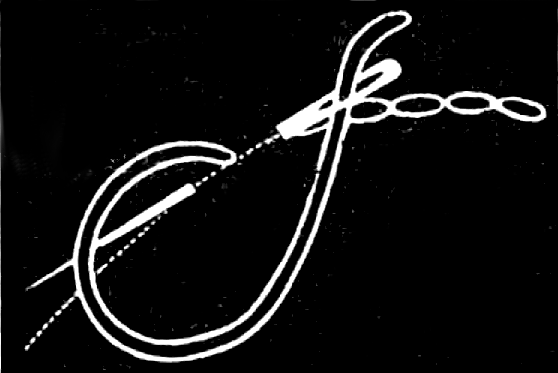
\includegraphics[keepaspectratio,width=\textwidth,height=0.75\textheight]{1.png}\\
Retroira\end{center}

\begin{center}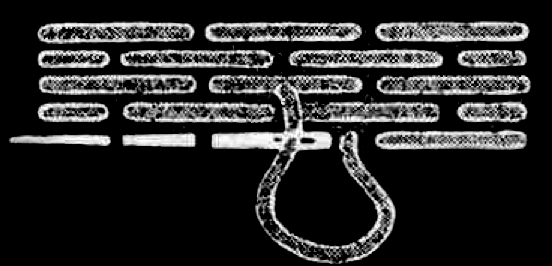
\includegraphics[keepaspectratio,width=\textwidth,height=0.75\textheight]{2.png}\\
Pleniga\end{center}

\begin{center}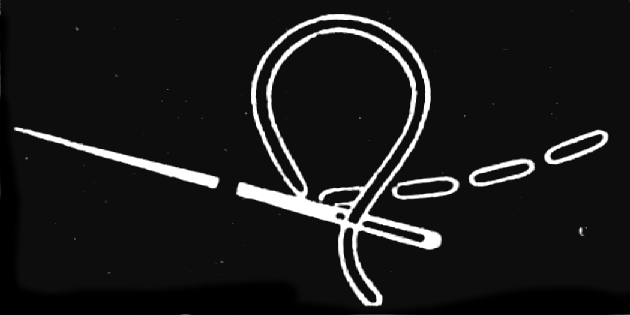
\includegraphics[keepaspectratio,width=\textwidth,height=0.75\textheight]{3.png}\\
Galopa aŭ Kuranta\end{center}

\begin{center}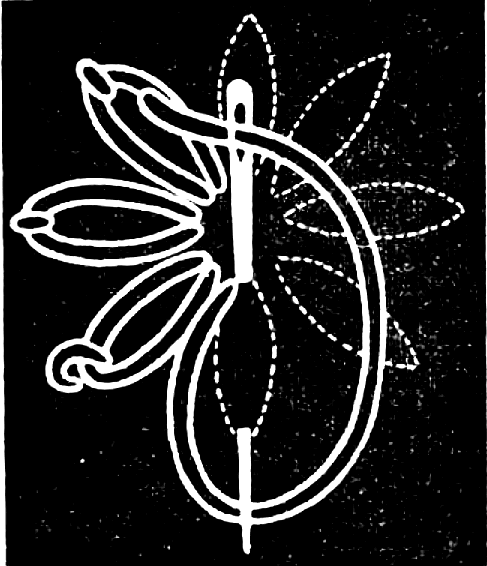
\includegraphics[keepaspectratio,width=\textwidth,height=0.75\textheight]{4.png}\\
Petala\end{center}

\begin{center}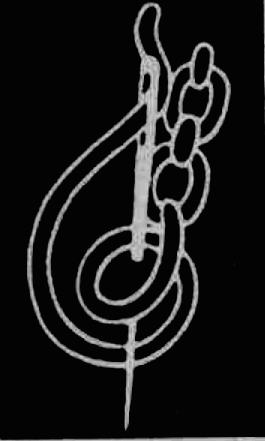
\includegraphics[keepaspectratio,width=\textwidth,height=0.75\textheight]{5.png}\\
Ĉena\end{center}

\begin{center}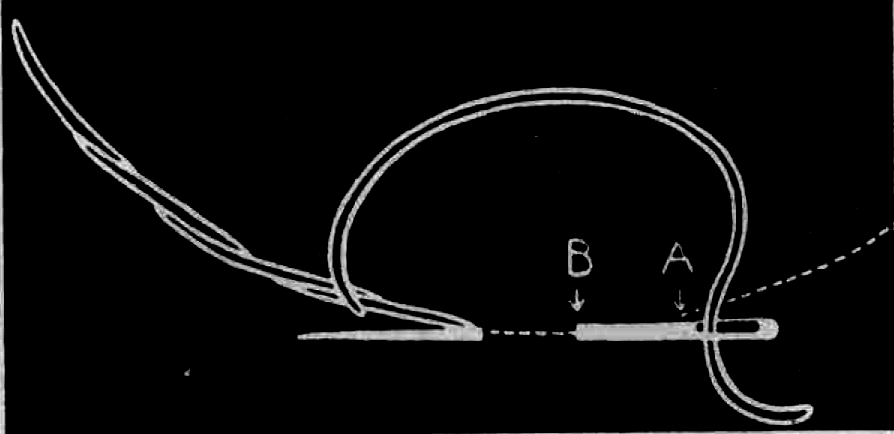
\includegraphics[keepaspectratio,width=\textwidth,height=0.75\textheight]{6.png}\\
Kontura\end{center}

\begin{center}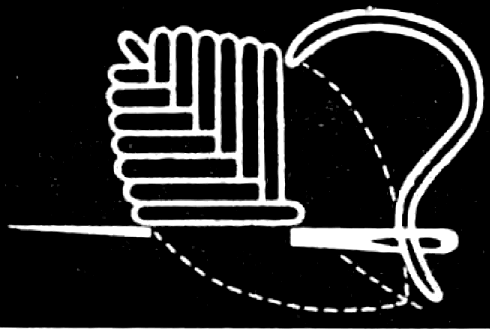
\includegraphics[keepaspectratio,width=\textwidth,height=0.75\textheight]{7.png}\\
Fiŝata (ank. Pleniga)\end{center}

\begin{center}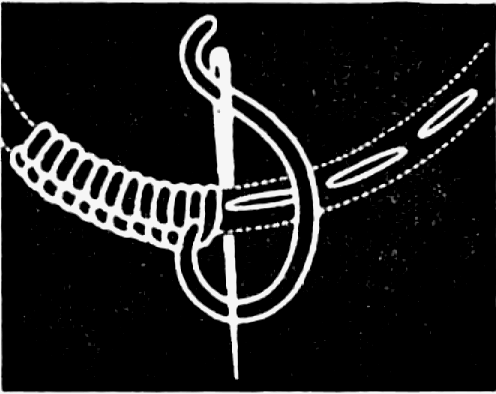
\includegraphics[keepaspectratio,width=\textwidth,height=0.75\textheight]{8.png}\\
Rand(bind)a\\
pli densa, meze sur ŝtofo\end{center}

\begin{center}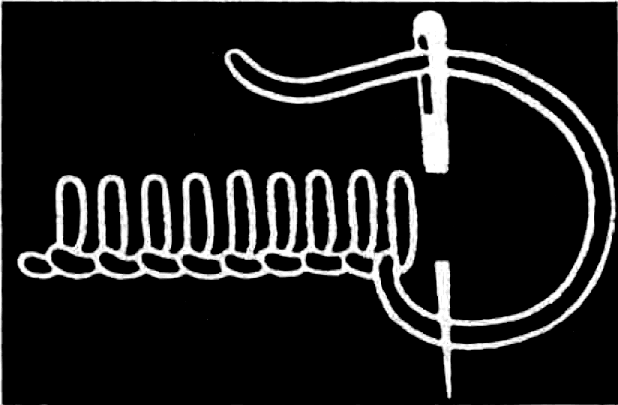
\includegraphics[keepaspectratio,width=\textwidth,height=0.75\textheight]{9.png}\\
Rand(bind)a\end{center}

\begin{center}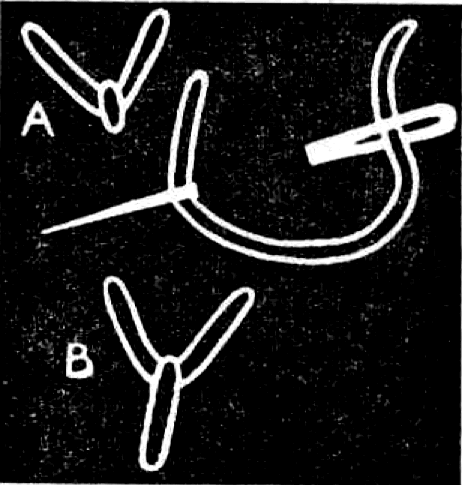
\includegraphics[keepaspectratio,width=\textwidth,height=0.75\textheight]{10.png}\\
Muŝpaŝoj aŭ Kokspuro\end{center}

\begin{center}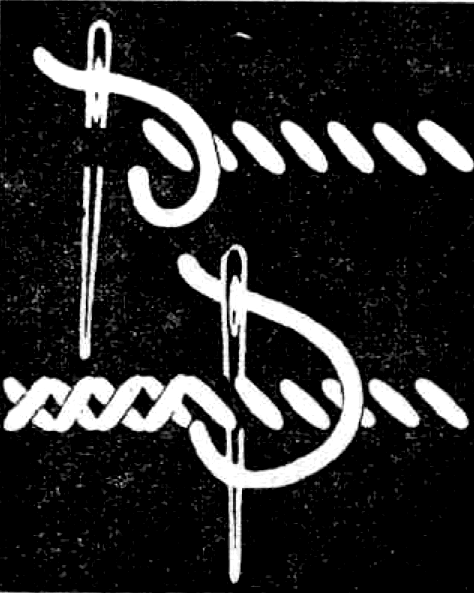
\includegraphics[keepaspectratio,width=\textwidth,height=0.75\textheight]{11.png}\\
Kruca\end{center}

\begin{center}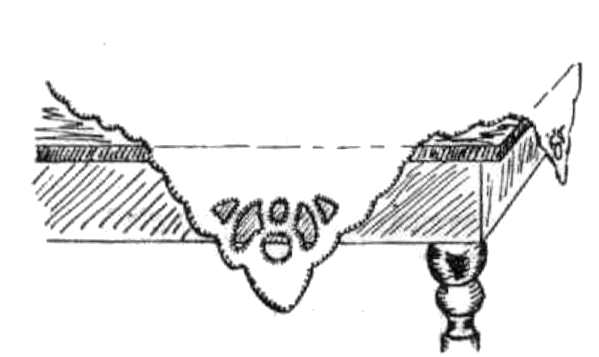
\includegraphics[keepaspectratio,width=\textwidth,height=0.75\textheight]{12.png}\\
Tajlita Tablotuko\end{center}

\begin{center}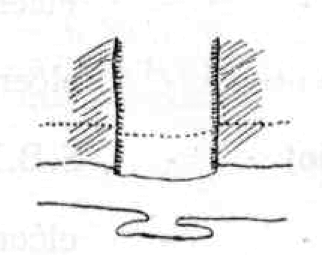
\includegraphics[keepaspectratio,width=\textwidth,height=0.75\textheight]{13.png}\\
Orlo de jupo montranta dufaldon (eksteran)\end{center}

\begin{center}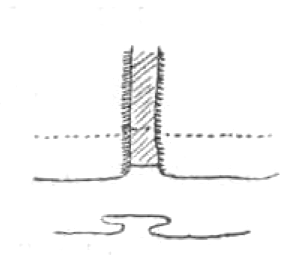
\includegraphics[keepaspectratio,width=\textwidth,height=0.75\textheight]{14.png}\\
Juporlo montranta dufaldon (interan)\end{center}

\begin{center}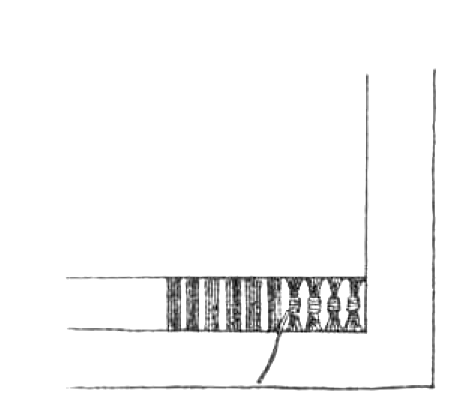
\includegraphics[keepaspectratio,width=\textwidth,height=0.75\textheight]{15.png}\\
Faskoj\end{center}

\chapter[Mallongigoj]{Mallongigoj}


\begin{description}
\item[k.t.p.]

 kaj tiel plu

\item[k.c.]

 kaj cetere

\item[k.s.]

 kaj simile

\item[vd.]

 vidu
\end{description}

\newpage

\textbf{TERMINAROJ}

eldonitaj de U.E.A.

\textbf{1. Fervoja Terminaro}		-	elĉerpita

\textbf{2. Armea Terminaro}		-	elĉerpita

\textbf{3. Aeronaŭtika Terminaro}		-	elĉerpita

\textbf{4. Terminaro por Infanludoj}		-	S.B.E.T.

\textbf{5. Radio-Terminaro}		-	elĉerpita

\textbf{6. Muzika Terminaro}	-		Butler kaj Merrick

\textbf{7. Filatela Terminaro}	-		H.M. Scott

\textbf{8 Leĝa Terminaro}		-	A.Mildwurf

\textbf{9. Kudra kaj Trika Terminaro}			M. kaj V. Verda

N-roj 4 kaj 6--9 ankoraŭ haveblaj ĉe U.E.A. po 10 pencoj aŭ 3 respondkuponoj afrankite.

\newpage
\begin{center}
			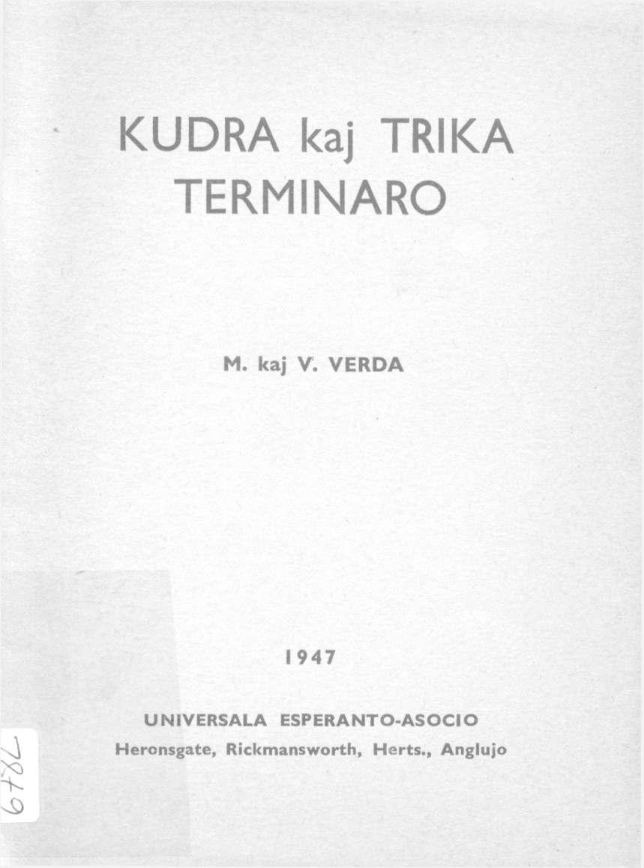
\includegraphics[width=1\textwidth]{titlopagho.pdf}
			\end{center}

\newpage\vspace*{\fill}\begin{center}

\emph{Printed by Sumfield}\\
\emph{Day Ltd Eastboume, England}\\
\emph{(36492)}

\end{center}
\vspace*{\fill}

%
%	MultiMarkdown default footer
%


% Back Matter
\if@mainmatter
	we're in main
	\backmatter
\fi


% Bibliography

\ifx\bibliocommand\undefined
\else
	\bibliographystyle{\bibliostyle}
	\bibliocommand
\fi



% Glossary
\printglossary[type=main,style=long,nonumberlist,title=Mallongigoj, toctitle=Mallongigoj]


% Index
\printindex


\end{document}
